\newpage
\appendix
\begin{figure}[H]
  \centering
	\begin{subfigure}{.496\linewidth}
		\centering
		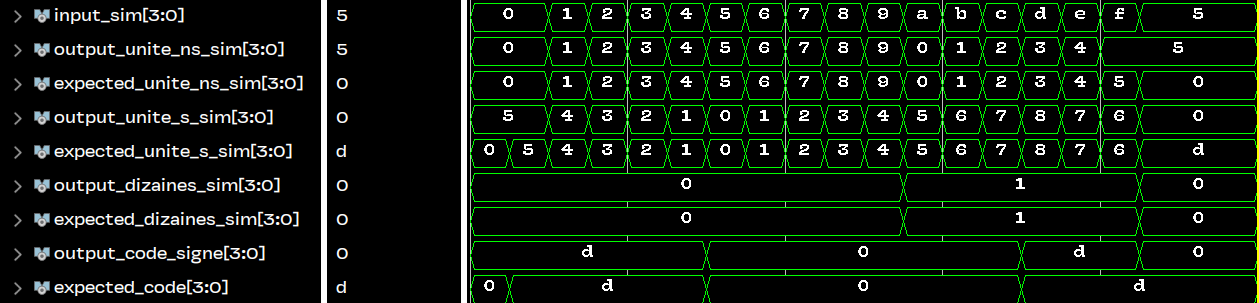
\includegraphics[width=\textwidth]{figures/img/graph-bin2dualbcd.png}
		\caption{Bin2DualBCD}
	\end{subfigure}
	\begin{subfigure}{.496\linewidth}
		\centering
		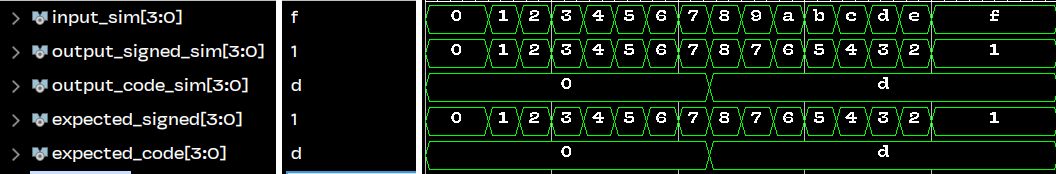
\includegraphics[width=\textwidth]{figures/img/graph-bin2dualbcd-signed.png}
		\caption{graph-bin2dualbcd-signed}
	\end{subfigure}
	\begin{subfigure}{.496\linewidth}
		\centering
		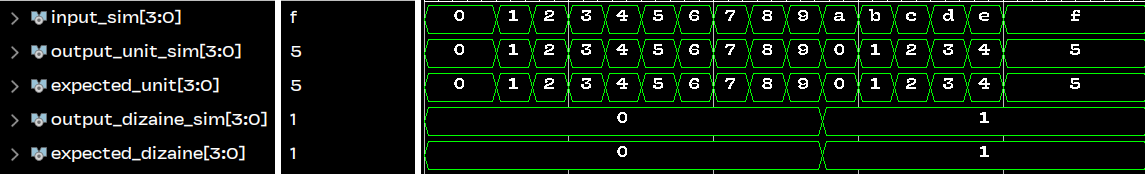
\includegraphics[width=\textwidth]{figures/img/graph-bin2dualbcd-unsigned.png}
		\caption{graph-bin2dualbcd-unsigned}
	\end{subfigure}
	\begin{subfigure}{.496\linewidth}
		\centering
		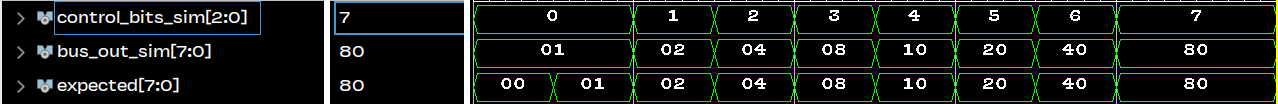
\includegraphics[width=\textwidth]{figures/img/graph-dec-2-a-8.png}
		\caption{graph-dec-2-a-8}
	\end{subfigure}
	\begin{subfigure}{.496\linewidth}
		\centering
		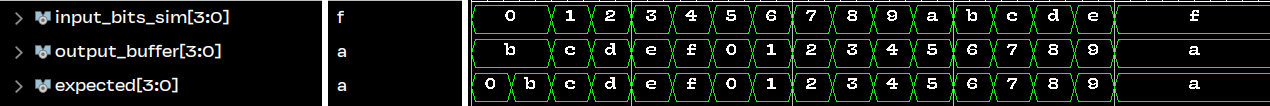
\includegraphics[width=\textwidth]{figures/img/graph-moins5.png}
		\caption{graph-moins5}
	\end{subfigure}
	\begin{subfigure}{.496\linewidth}
		\centering
		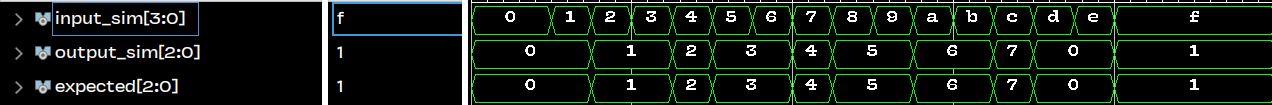
\includegraphics[width=\textwidth]{figures/img/graph-mult-2-3.png}
		\caption{graph-mult-2-3}
	\end{subfigure}
	\begin{subfigure}{.496\linewidth}
		\centering
		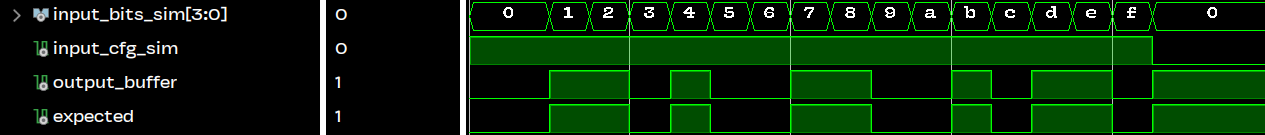
\includegraphics[width=\textwidth]{figures/img/graph-parite-pressed.png}
		\caption{graph-parite-pressed}
	\end{subfigure}
	\begin{subfigure}{.496\linewidth}
		\centering
		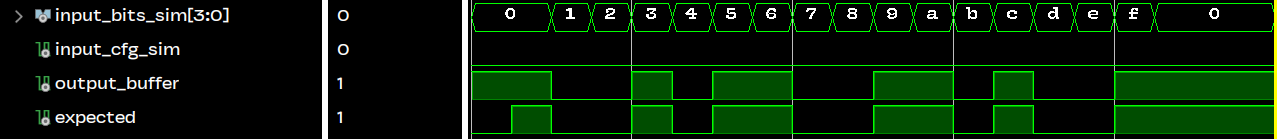
\includegraphics[width=\textwidth]{figures/img/graph-parite-unpressed.png}
		\caption{graph-parite-unpressed}
	\end{subfigure}
	\begin{subfigure}{.49\linewidth}
		\centering
		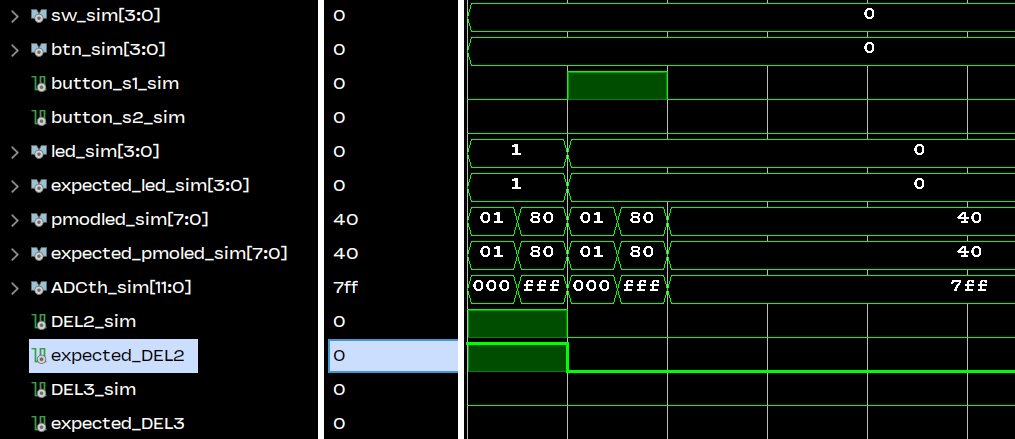
\includegraphics[width=\textwidth]{figures/img/graph-appcombitop.png}
		\caption{graph-appcombitop}
	\end{subfigure}
	\begin{subfigure}{.496\linewidth}
		\centering
		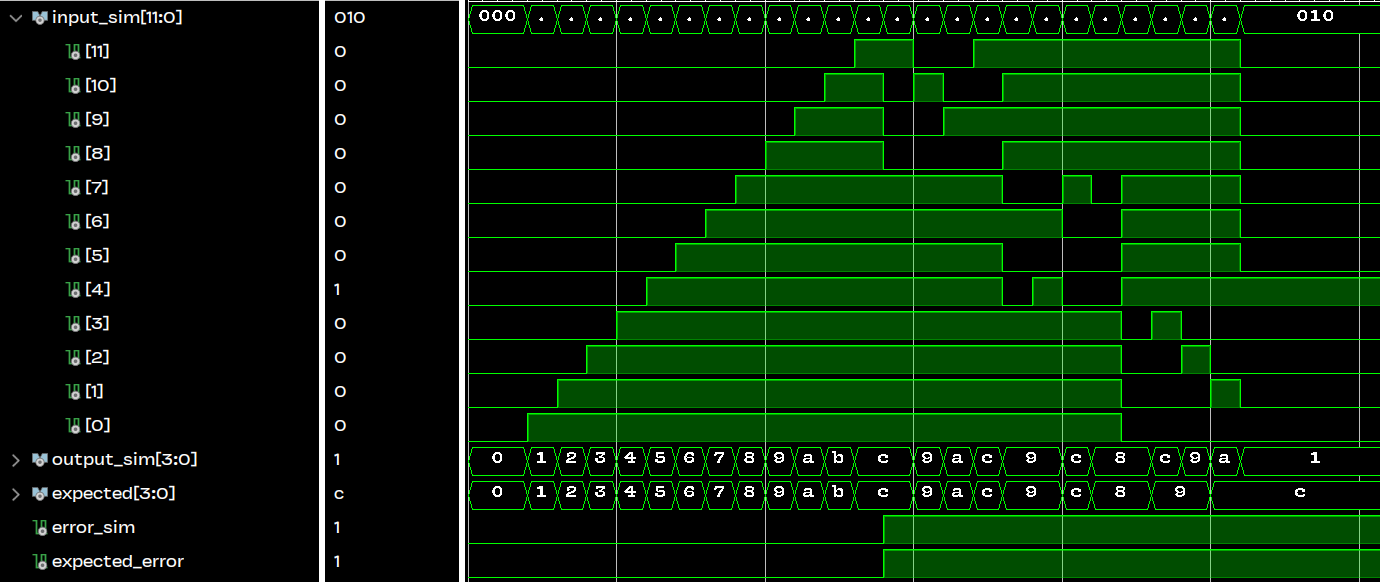
\includegraphics[width=\textwidth]{figures/img/graph-thermo2bin.png}
		\caption{graph-thermo2bin}
	\end{subfigure}
	\begin{subfigure}{.496\linewidth}
		\centering
		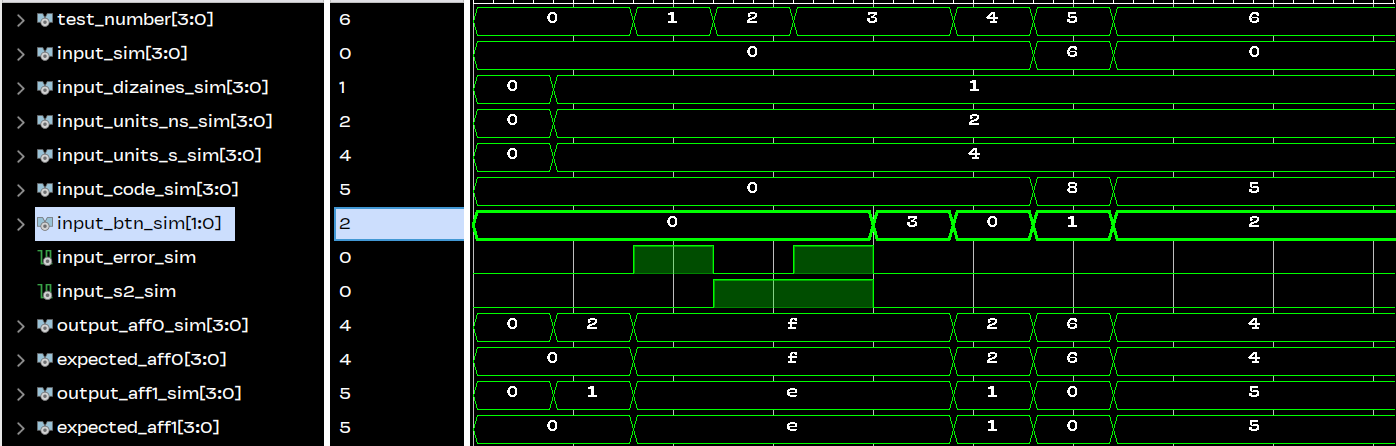
\includegraphics[width=\textwidth]{figures/img/graph-mux.png}
		\caption{graph-mux}
	\end{subfigure}
	\caption{Chronogrames des simulations Vivado}
\end{figure}



\section{Code VHDL}

\begin{figure}[H]
	\tiny
	\centering
	\begin{varwidth}{\linewidth}
		\input{figures/code/thermo2bin.tex}
	\end{varwidth}
	\caption{Module Thermo2bin}
\end{figure}

\begin{figure}[H]
	\tiny
	\centering
	\begin{varwidth}{\linewidth}
		\input{figures/code/add4bits.tex}
	\end{varwidth}
	\caption{Module Add4Bits}
\end{figure}

\begin{figure}[H]
	\tiny
	\centering
	\begin{varwidth}{\linewidth}
		\input{figures/code/add1bita.tex}
	\end{varwidth}
	\caption{Module Add1BitA}
\end{figure}

\begin{figure}[H]
	\tiny
	\centering
	\begin{varwidth}{\linewidth}
		\input{figures/code/add1bitb.tex}
	\end{varwidth}
	\caption{Module Add1BitB}
\end{figure}

\section{Schémas Bloc}

\begin{figure}[H]
	\centering
	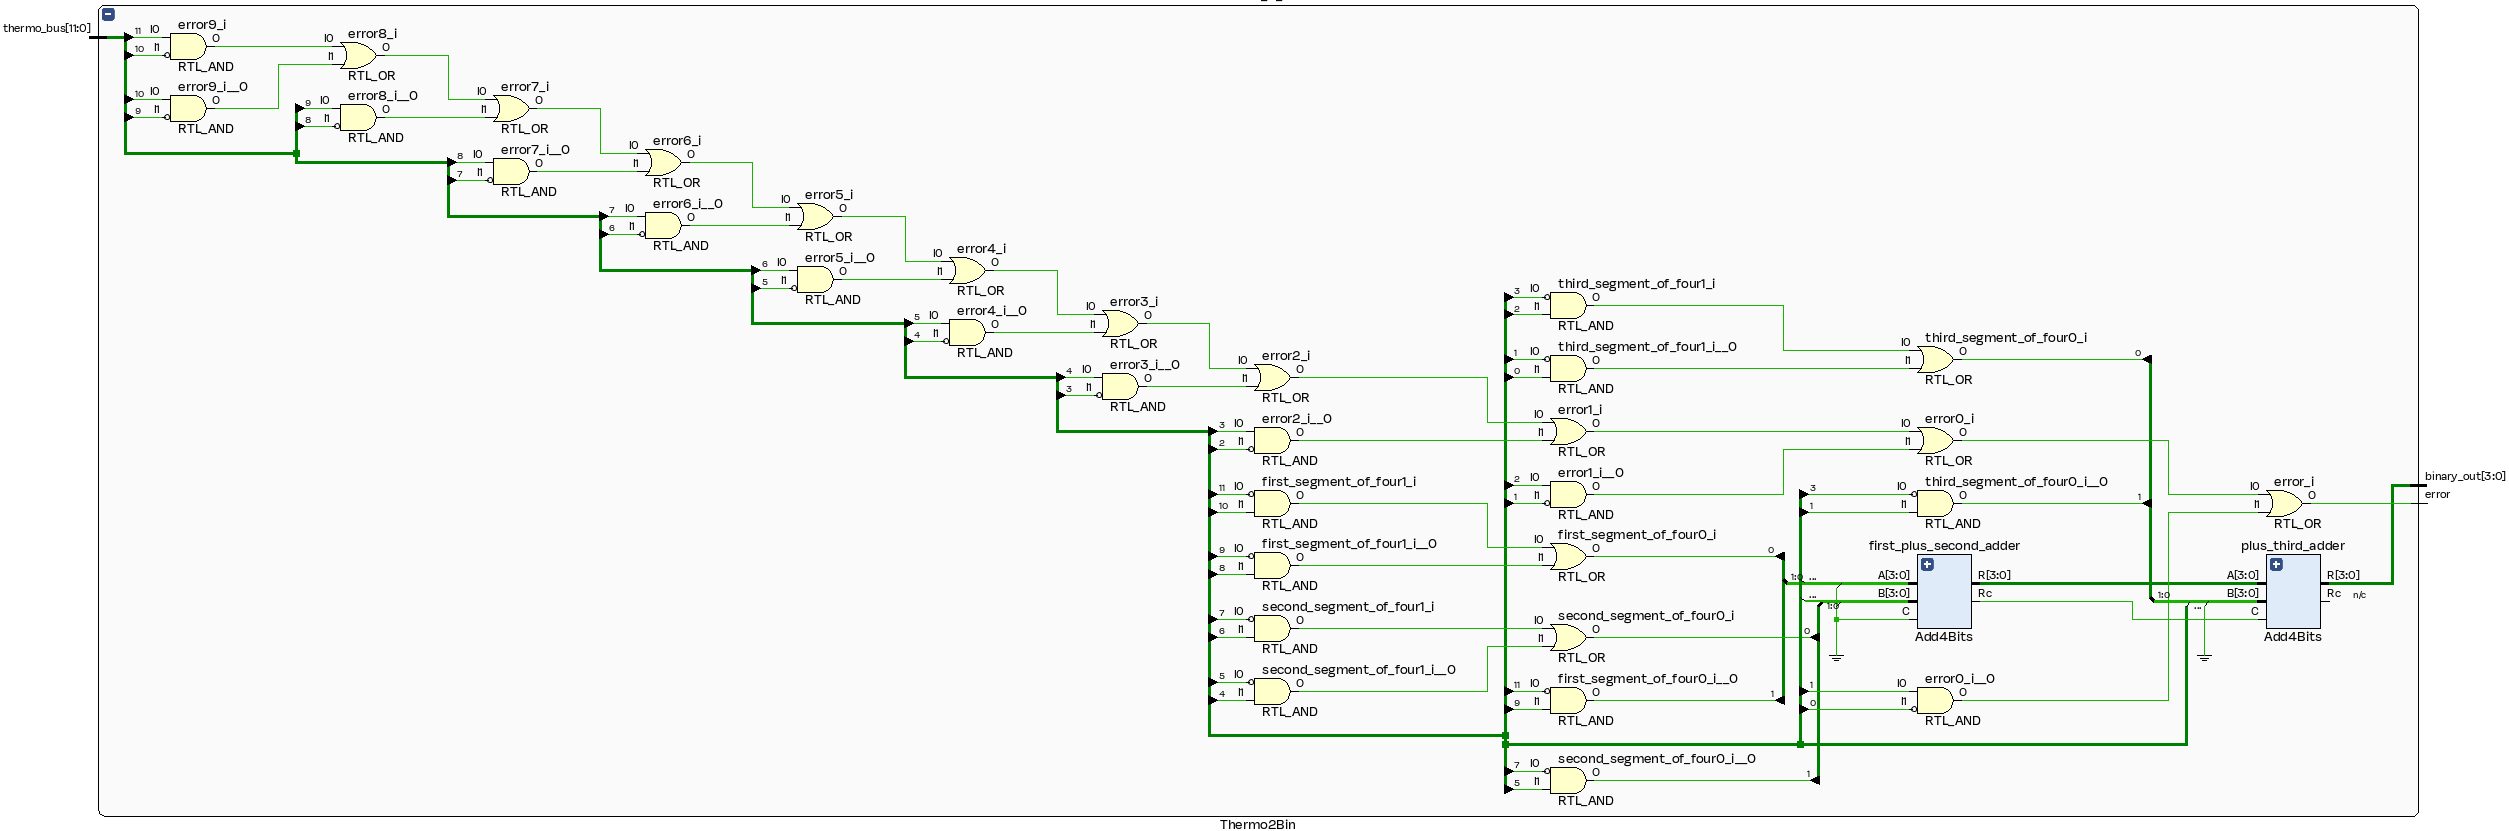
\includegraphics[width=\textwidth]{figures/img/schematic-thermo2bin.png}
	\caption{Module Thermo2bin}
\end{figure}

\begin{figure}[H]
	\centering
	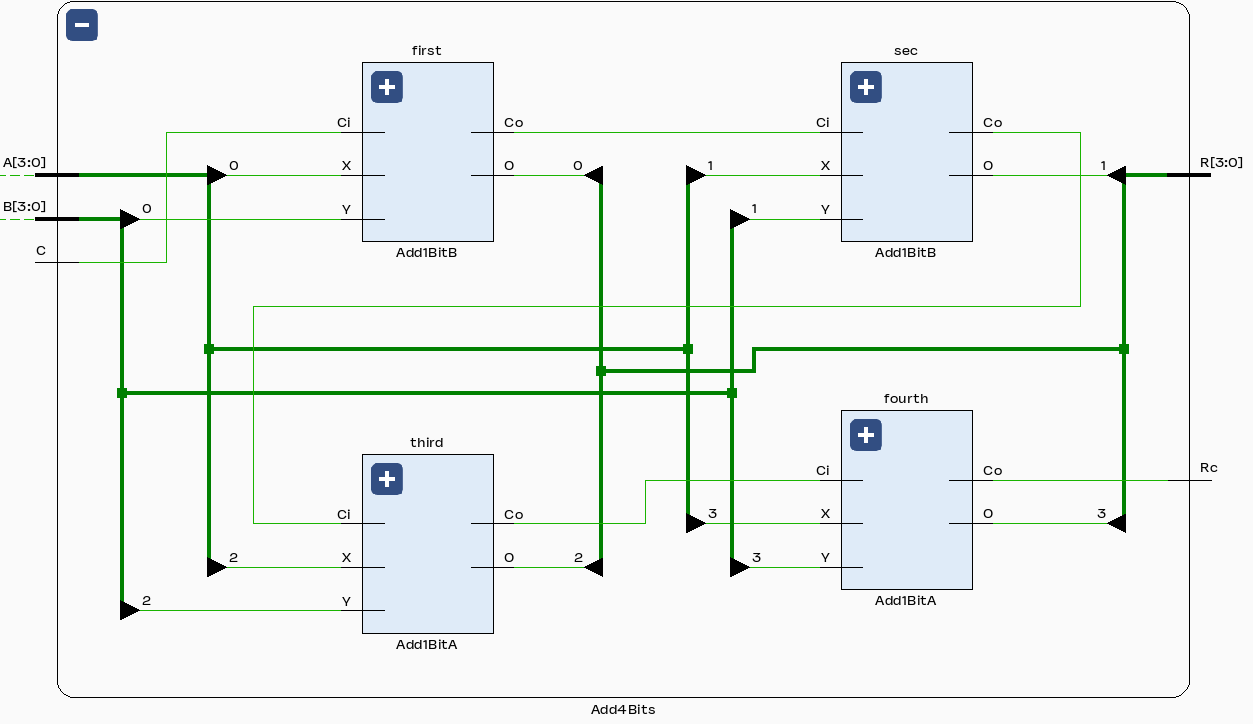
\includegraphics[width=.6\textwidth]{figures/img/schematic-add4bits.png}
	\caption{Module Add4Bits}
\end{figure}

\begin{figure}[H]
	\centering
	\begin{subfigure}{0.60 \linewidth}
		\centering
		\vfill
		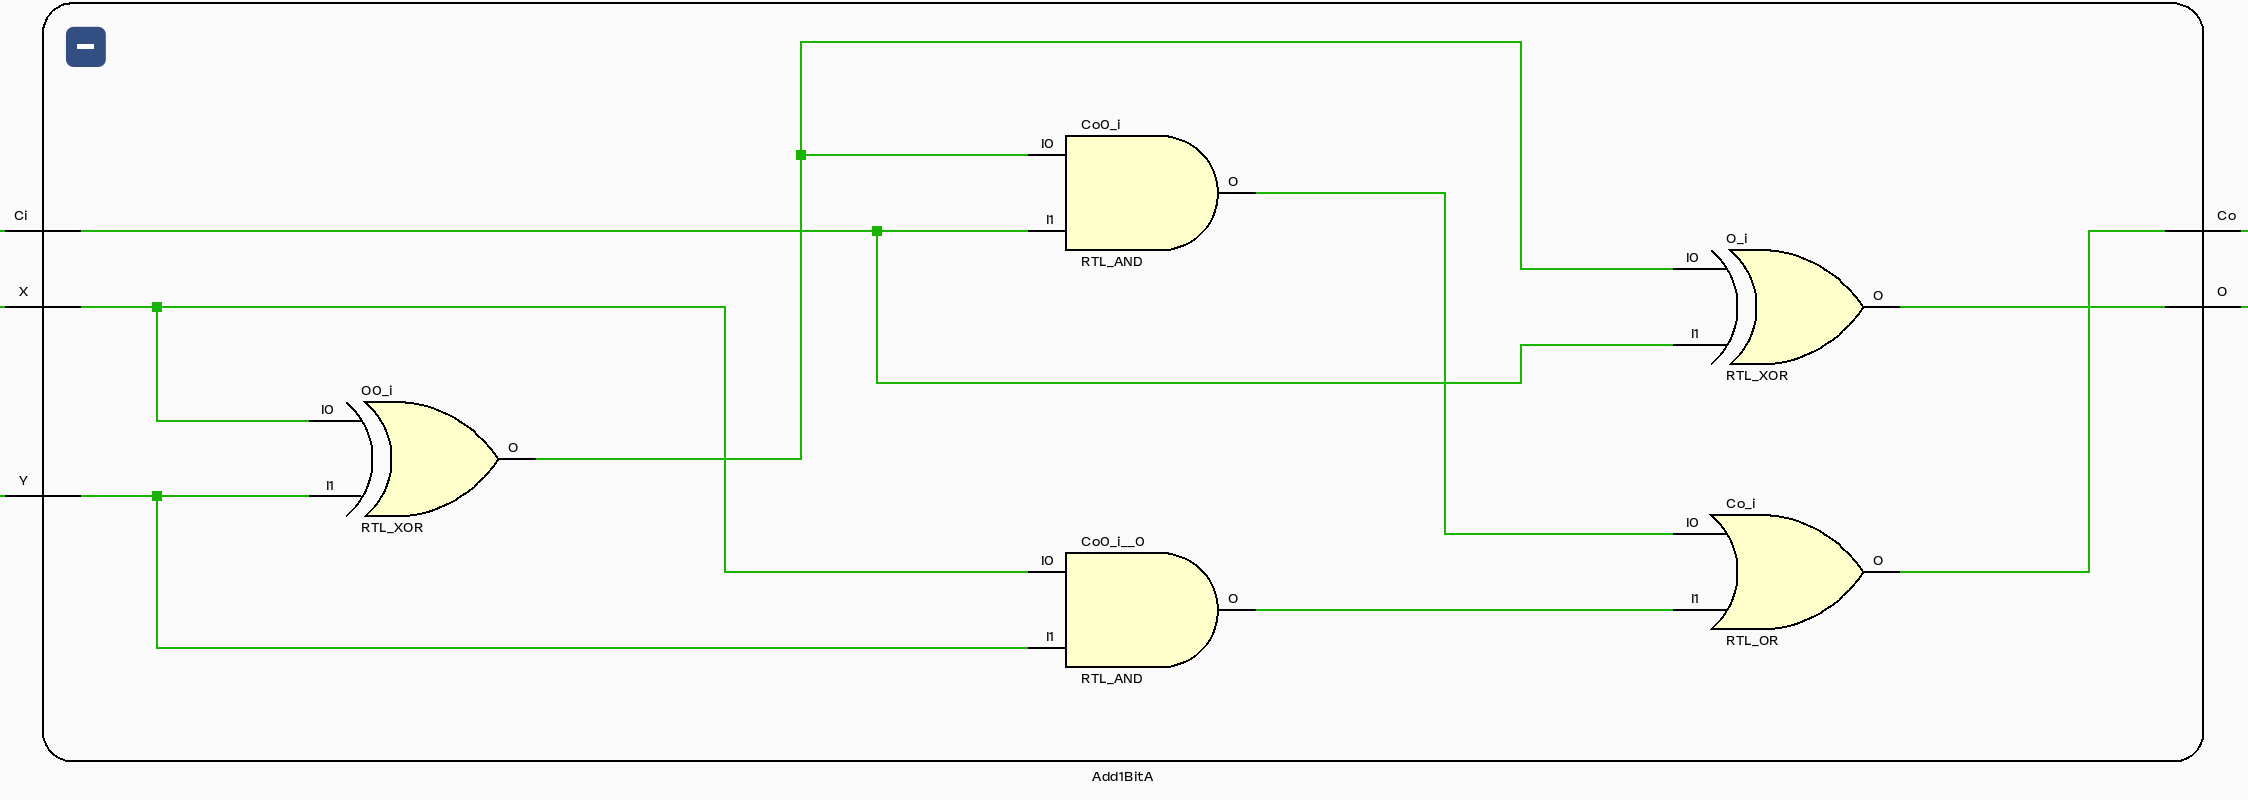
\includegraphics[width=\textwidth]{figures/img/schematic-add1bita.png}
		\caption{Add1BitA: Conception parallèle}
	\end{subfigure} \hfill
	\begin{subfigure}{0.39 \linewidth}
		\centering
		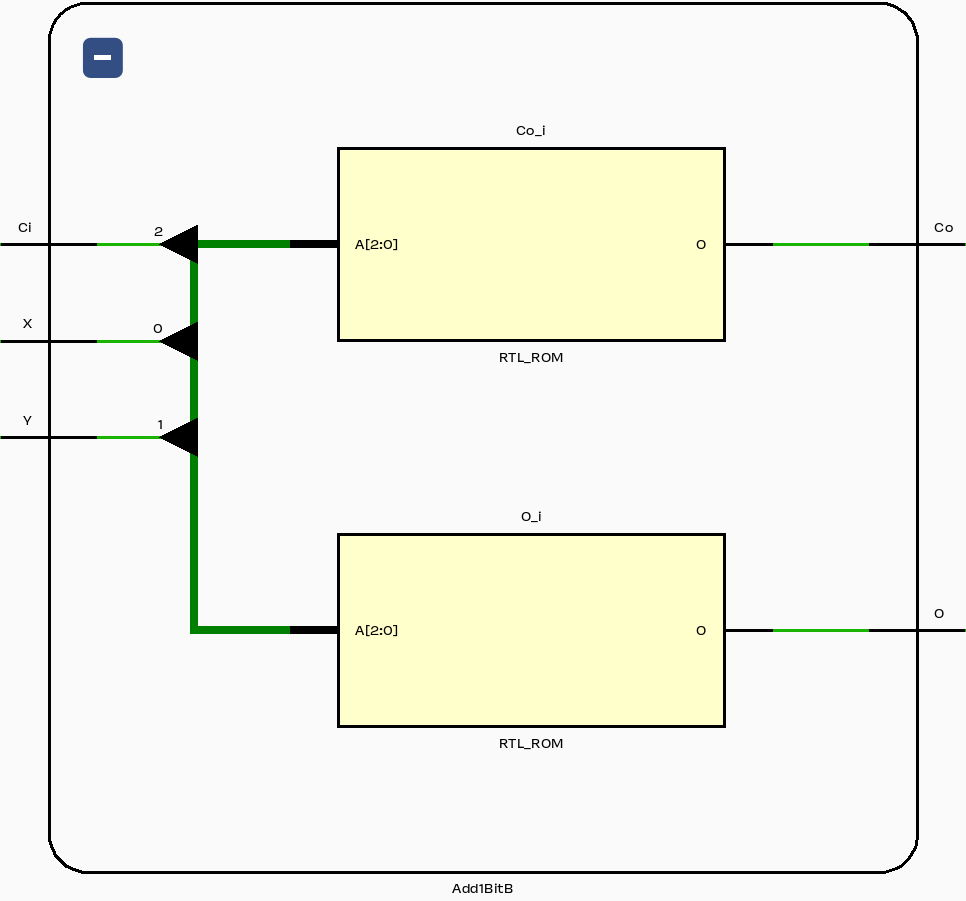
\includegraphics[width=\textwidth]{figures/img/schematic-add1bitb.png}
		\caption{Conception séquentielle avec \textit{CASE}}
	\end{subfigure}
	\caption{Additionneurs 1 bit}
\end{figure}


\section{Tables de Vérité et Karnaugh}

\begin{table}[H]
	\centering
	\caption{Table de vérité des Bits}
	\label{tab:table-de-vérité-thermométrique-4-bits}
	\vspace{.2cm}
	\begin{tabular}{llllllll}
		\toprule
		A & B & C & D & E & F & G & H \\
		\midrule
		0 & 0 & 0 & 0 & 0 & 0 & 0 & 0 \\
		0 & 0 & 0 & 1 & 0 & 0 & 0 & 1 \\
		0 & 0 & 1 & 1 & 0 & 0 & 1 & 0 \\
		0 & 1 & 1 & 1 & 0 & 0 & 1 & 1 \\
		1 & 1 & 1 & 1 & 0 & 1 & 0 & 0 \\
		\bottomrule
	\end{tabular}

\end{table}

% \begin{figure}[H]
% \centering
% \begin{karnaugh-map}[4][4][1][$D$][$C$][$B$][$A$]
% \manualterms{
%   0,1,2,3,
%   4,5,6,7,
%   8,9,10,11,
%   12,13,14,15
% }
% \implicant{1}{9}
% \implicant{4}{6}
% \end{karnaugh-map}
% \caption{Karnaugh pour le bit $H$}
% \end{figure}
%
\begin{figure}[H]
\centering
\begin{karnaugh-map}[4][4][1][$D$][$C$][$B$][$A$]
\manualterms{
	0,1,X,0,
	X,X,X,1,
	X,X,X,X,
	X,X,X,0}
\implicant{1}{9}
\implicant{4}{6}
\end{karnaugh-map}
\caption{Karnaugh pour le bit $H$}
\label{tab:karnaugh-bit-H}
\end{figure}

\begin{figure}[H]
\centering
\begin{karnaugh-map}[4][4][1][$D$][$C$][$B$][$A$]
\manualterms{
	0,0,X,1,
	X,X,X,1,
	X,X,X,X,
	X,X,X,0}
\implicant{3}{6}
\end{karnaugh-map}
\caption{Karnaugh pour le bit $G$}
\label{tab:karnaugh-bit-G}
\end{figure}

